% Lauren DeDieu, Jerrod M.~Smith, Kimberly Golubeva and Christian Bagshaw
% A Resource Bank for Writing Intensive Mathematics Courses
% This work is licensed under a  Creative Commons Attribution-NonCommercial-ShareAlike 4.0 International License
% http://creativecommons.org/licenses/by-nc-sa/4.0/
%-----------------%-----------------
\section{Overview of error classification}\label{sec-error}
%-----------------%-----------------
For each of the Flawed Proofs in Part \ref{part-proofs}, we include a classification of the errors contained therein using Strickland and Rand's Proof-Error Coding Scheme:

%\cite[Figure 1]{Strickland_2016} (see Figure \ref{fig-sr-err}).

% Figure included with the permission of Strickland and Rand
\begin{figure}[h] %remove [h] to allow the figure to `float'
\caption{Strickland and Rand's Proof-Error Coding Scheme \cite[Figure 1]{Strickland_2016}}\label{fig-sr-err}
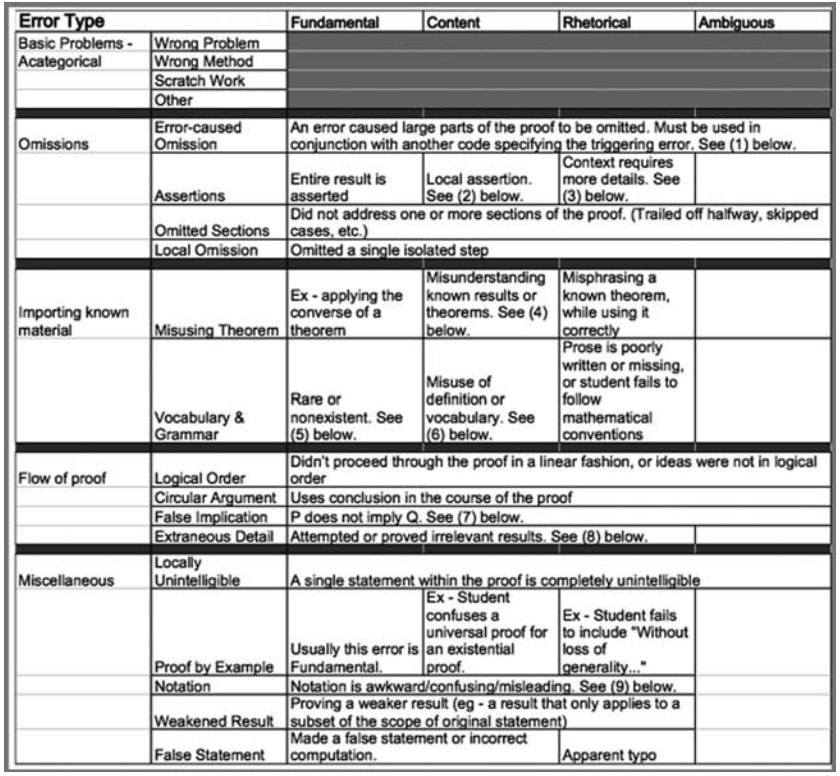
\includegraphics[width=\linewidth]{Error/Strickland&Rand_CodingSchemeMatrix(Fig1_PRIMUS_26_10_905-921)}
\end{figure}

The rows of the coding scheme represent the type of error and the columns represent the severity of the error. Please refer to the Appendix of \cite[Figure 1]{Strickland_2016} for a more detailed description of these error classifications.

\subsection{Abbreviated Error Codes}
To streamline the use of the error classification we will use the following system for abbreviating the error classifications:

%Error types will be read from Figure \ref{fig-sr-err} as ``Column Row", i.e., ``Severity Type". For instance, we may encounter a ``Content Misusing Theorem'' error or a ``Fundamental Logical Order'' error. This convention informs the following system of abbreviations:

\begin{figure}[h]
\caption{`Severity of error' codes}\label{fig-code-severe}
\begin{multicols}{2}
\begin{description}
\item[F] Fundamental	
\item[C] Content
\item[N] Novice \footnotemark
\item[A] Ambiguous
\end{description}
\end{multicols}
\end{figure}

\footnotetext{In this document, we use ``Novice'' in place of Strickland and Rand's descriptor ``Rhetorical". }

%\vspace{-0.75cm}

\begin{figure}[h]
\caption{`Type of error' codes}\label{fig-code-type}
\begin{multicols}{2}
\begin{description}
\item[WP] Wrong Problem
\item[WM] Wrong Method
\item[SW] Scratch Work
\item[EO] Error-caused Omission \footnotemark
\item[A] Assertions
\item[OS] Omitted Sections
\item[O] Omission / Local Omission
\item[MT] Misusing Theorem
\item[VG] Vocabulary \& Grammar
\item[Log] Logical Order
\item[Cir] Circular Argument
\item[FI] False Implication
\item[ED] Extraneous Detail
\item[LU] Locally Unintelligible
\item[Eg] Proof by Example
\item[N] Notation
\item[WR] Weakened Result
\item[FS] False Statement
%\item[Misc] Miscellaneous / Other
\end{description}
\end{multicols}
\end{figure}

\footnotetext{Note that the Error-caused Omission code must always be used in conjunction with a second error type (and severity) code for the original error that caused the subsequent omission. We will use a hyphen/parentheses to indicate such an error. For example, if an omission occurred as a result of misunderstanding a known theorem. this would be an Error-caused Omission resulting from a Content Misusing Theorem error, and it would be abbreviated as EO-(C-MT).}

For example, using these abbreviations, a Content Misusing Theorem error will be abbreviated by C-MT and a Fundamental Logical Order error will be abbreviated by F-Log. Using Strickland and Rand's scheme, the errors Wrong Problem, Wrong Method, and Scratch Work do not have severity ratings.



%%%%% I removed the below now about MISC because it looks like we don't use MISC anywhere in this document. I also commented it out above.

%Moreover, our use of `Miscellaneous' is different from Strickland and Rand's but agrees with their use of `Other' \cite{Strickland_2016}.



